\section{Personalization of Cardiac Biomechanics}
\label{sec:intro_personalization}
In this section we will go through the steps needed to personalize the
mechanical models developed in the previous section towards a given
patient. We will start by giving a brief overview of the
interaction between medical imaging and cardiac computational model.
Then we will explain how the geometries are extracted from the
medical images and turned into a computational mesh,  which we can use
for finite element computations. Finally we will explain how to
incorporate additional data into model by means of adjoint based data
assimilation techniques.


\subsection{Medical Imaging}

Since the discovery of X-ray in 1895, medical imaging has played a central
role in diagnosis, treatment planning and follow-up. Without the huge
advancements in medical imaging the last decades, computational models
would not have been as important and promising as it has become.


Cardiac computational modeling often relies on data obtained using
medical imaging techniques, and the quality of such data is therefore of
fundamental importance \cite{lamata2014images}. It is clear, that
without advancements in medical imaging technology, the role of
computational models would be limited to simple, idealized cases. With
access to high quality images, detailed information about cardiac structure
can be used to e.g build anatomically correct models. The
computational models can then later be validated agains this images,
or we can assimilate additional data extracted from this images to
extract biomarkers. Figure \ref{fig:cardiac_imaging_model} summarizes
this interaction between medical images and computational models. 

\begin{figure}[htbp]
  \centering
    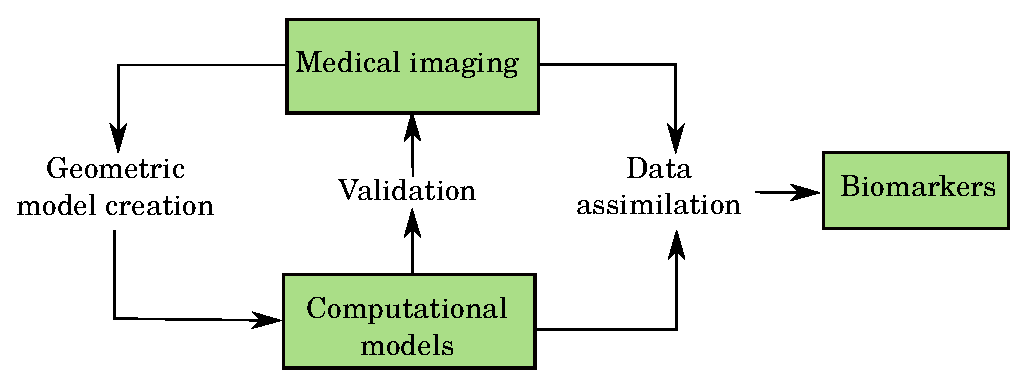
\includegraphics[width=\textwidth]{chapters/introduction/figures/models.eps}
\caption{Interaction between medical imaging and computational
  models. Medical images are used to extract geometric
  structure. These geometries together with the computational models
  can later be validated against the medical images. Computational
  models can also be used togther with the medical images to
  assimilate additional data in order to extraction clinically useful
  biomarkers. }
\label{fig:cardiac_imaging_model}
\end{figure}



% Still, one of the major bottlenecks in terms of personalized
% computaional models is the quality of data (and representations of
% model). There is a big issue in
% reproducebility, because of noisy data, and operator depedent
% measurements.
Today there are three main non-invasive imaging techniques used in
cardiology. These are chocardiography (Echo), magnetic
resonance imaging (MRI) and computed tomography (CT). Each
modality offers advantages and disadvatages over the other

For example, MRI provides
high quality images, uses zero radiation, but is exspensive and lacks
temporal resolution. CT can more accuratley reconstruct the 3D image
in contrast to MRI, in which 2D slices needs to be glued together to
form a 3D surface. However, CT exposes the patient to radiation which
increases the chance of developing cancer. Finally echocardiography is
easy to use, cheap, harmless, and  has good temporal resolution, but
is clearly inferior when it comes to image quality. 

% \subsubsection{EchoPac}

The main modality used in this thesis is 4D echocardiography, and we
will therefore focus on data aquired using this modality.
With 4D we mean three spatial and one temporal dimesion.
The speed of sound in human tissue (which is approxmately 1540 m/s)
put some limitations on the image quality verus the frame-rate
\cite{rabben2010technical} for these 3D volume images. In order to
increase the resolution, such an image is formed by stiching together
$N$ disjoint subvolumes aquired during $N$ cardiac cycles ($N$
typicall between 2 and 8)\cite{brekke2007volume}. 

The images are later processed using some image segmentation tool.
One such tool is EchoPac which is used for analysing images for GE
Vingmed. The 4D Auto LVQ tool in EchoPac, is a tool for processing 3D
echo images, and traces of volume, triangulated surfaces and 3D strain
\cite{heimdal20114d} traces together with a structured mesh of the
American Heart Association (AHA) segments
\cite{cerqueira2002standardized} for each time point, see Figure
\ref{fig:echopac_output}. 

\begin{figure}[htbp]
  \centering
  \begin{subfigure}[t]{0.3\textwidth}
    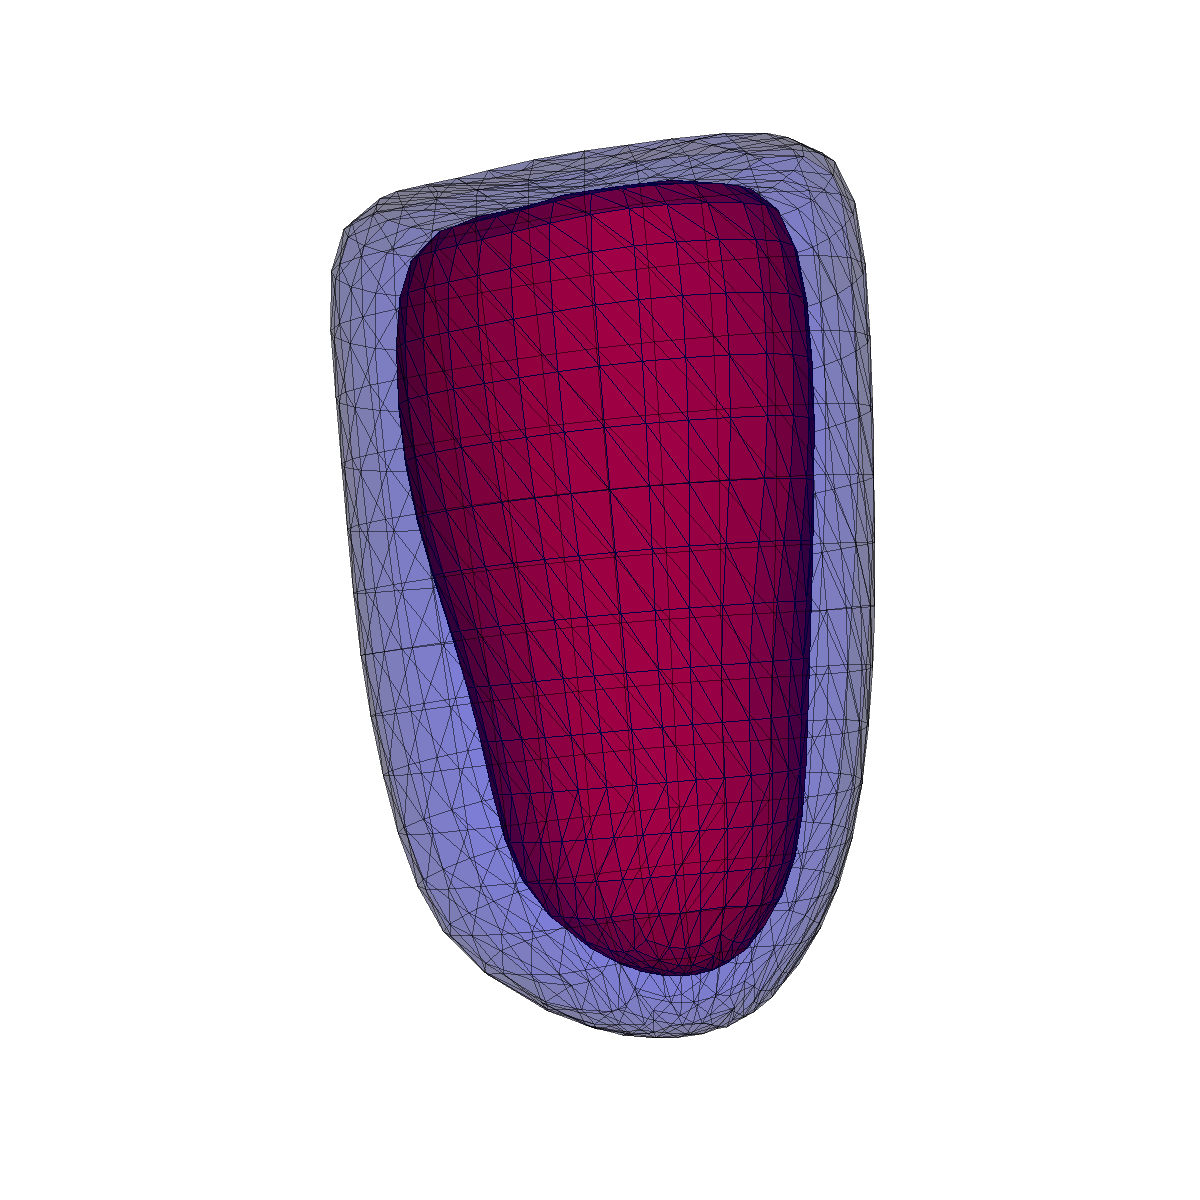
\includegraphics[width=\textwidth]{chapters/introduction/figures/geometry/raw.png}
    \caption{\label{fig:echopac_out_surf}}
  \end{subfigure}
  \begin{subfigure}[t]{0.3\textwidth}
    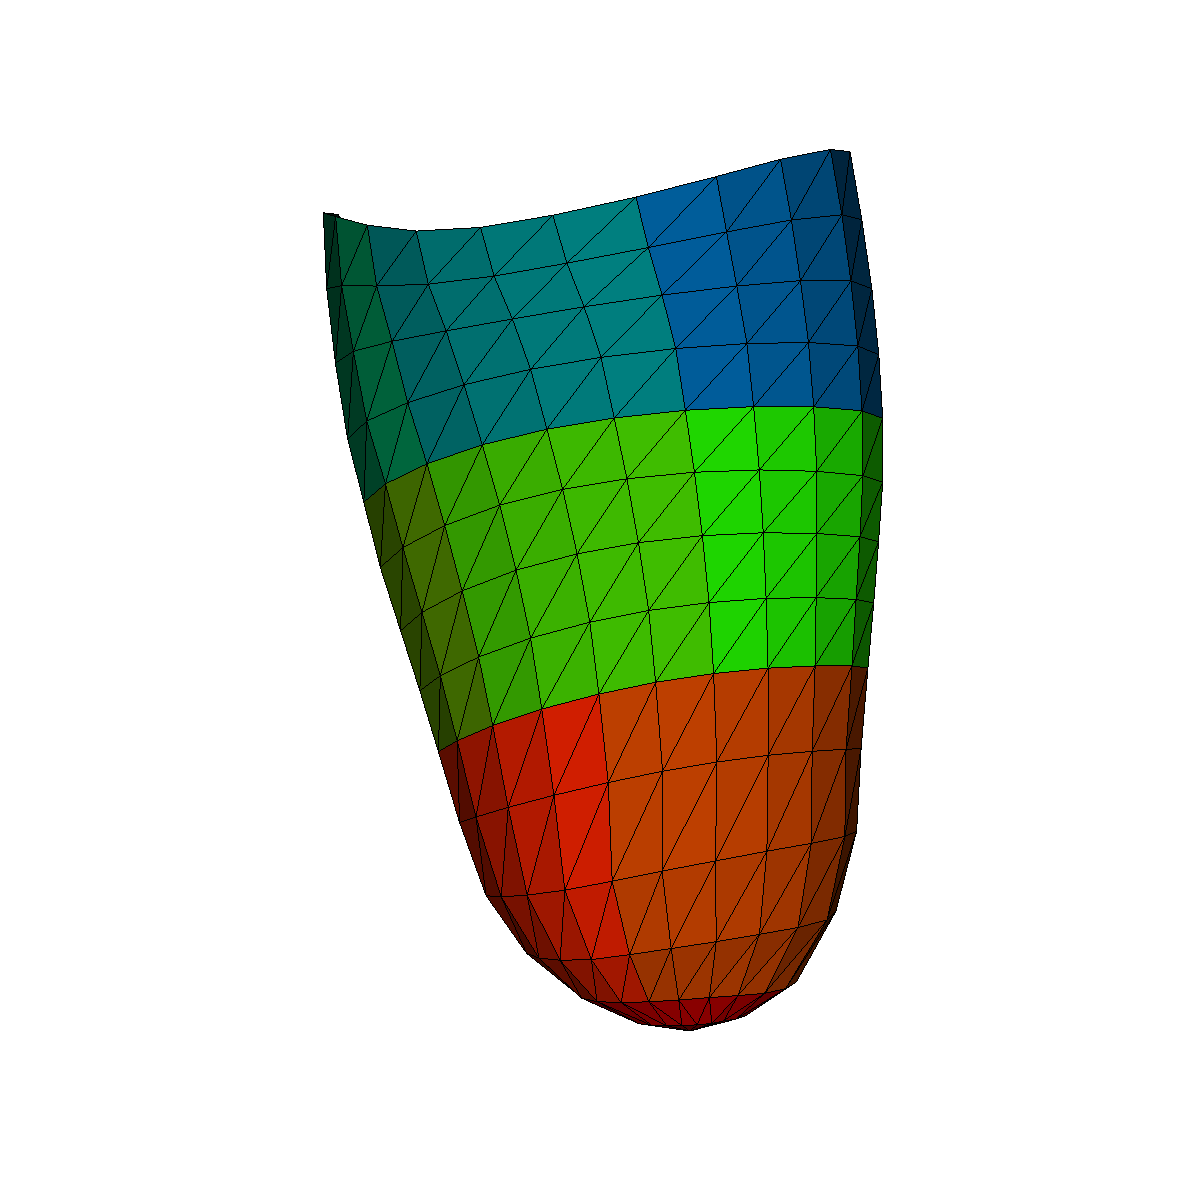
\includegraphics[width=\textwidth]{chapters/introduction/figures/geometry/strain_mesh.png}
    \caption{\label{fig:echopac_out_strain_mesh}}
  \end{subfigure}
  \begin{subfigure}[t]{0.38\textwidth}
    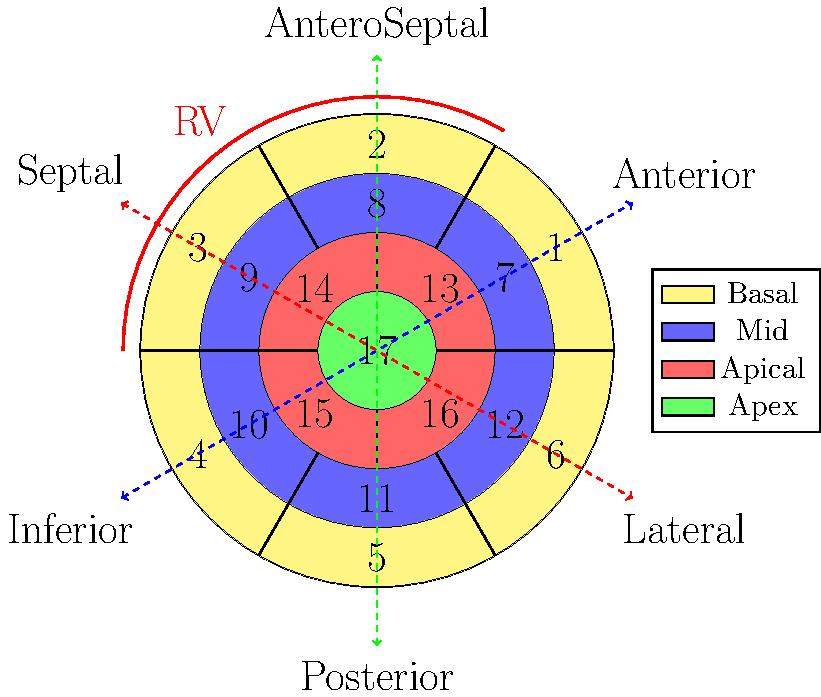
\includegraphics[width=\textwidth]{chapters/introduction/figures/bullseye/bullseye.pdf}
    \caption{\label{fig:bullseye_intro}}
  \end{subfigure}
\caption{Figure \ref{fig:echopac_out_surf} shows triangulated surfaces of the
      endo- and epicardium, and Figure
      \ref{fig:echopac_out_strain_mesh} shows structured mesh of the
      American Heart Association (AHA) segments. These surfaces are
      exported from the image segmentational tool EchoPac. Figure 
      \ref{fig:bullseye_intro} shows the American Heart Association (AHA)
      segments illustrated on a so called bullseye plot with name and
      numbers on the different segments. }
\label{fig:echopac_output}
\end{figure}


\subsection{Geometry and microstructure}


\subsubsection{Mesh generation}
In this section we will explain how to generate a left ventricular
mesh based on segmented surfaces coming from 4D echocardiography.
Figure \ref{fig:echopac_output} shows an example of how the exported data
from the image semgentation tool looks like. For each time point we
can extract triangulated surfaces of the endocardium and epicardium
which can be seen in Figure \ref{fig:echopac_out_surf}. Together with
these surfaces we are also given a so called strain mesh (Figure
\ref{fig:echopac_out_strain_mesh}) located approximately in the
midwall, which defines the approximate location of the AHA-segments
\cite{cerqueira2002standardized}, and can be used to orient the mesh. 



As discussed in \ref{sec:mech_boudary}, we constrain the basal movement in
the longitudinal direction, which is easiest to accomplished using a flat
base located at a prescribed location. In order to make the base flat
we first orient the surfaces so that the longitudinal axis is aligned
with the $x$-axis, and the apex pointing in the postive $x$
direction. To conststruct the basal plane we first take out the basal
points from the strain mesh, and use these points to construct a least
sqauare fitting plane (Figure \ref{fig:strain_mesh_plane}). Let $(x_i, y_i, z_i), i = 1, \cdots, N$
be the basal points, and suppose the basal plane solves the equation
$z = ax + by + c$, for some unknown constants $a,b,c$. Following a
least square approach, we select the parameters $(a,b,c)$ that
minimizes to sum
\begin{align}
  \sum_{i = 1}^{N} \left(ax_i + by_i + c  - z_i \right)^2.
\end{align}
Once the parameters for the basal plane is found we adjust the size of
the cut, by moving the plane along the longitudinal axis (here
$x-$axis), until the cavity volume agrees with the measured volume
given by the image segmentation tool within some specified tolerance. 
When the correct size is found the points above the plane is removed,
and the remaining surfaces are smoothed using the GAMer
\cite{yu2008feature}.

\begin{figure}[htbp]
  \centering
  \begin{subfigure}[t]{0.3\textwidth}
    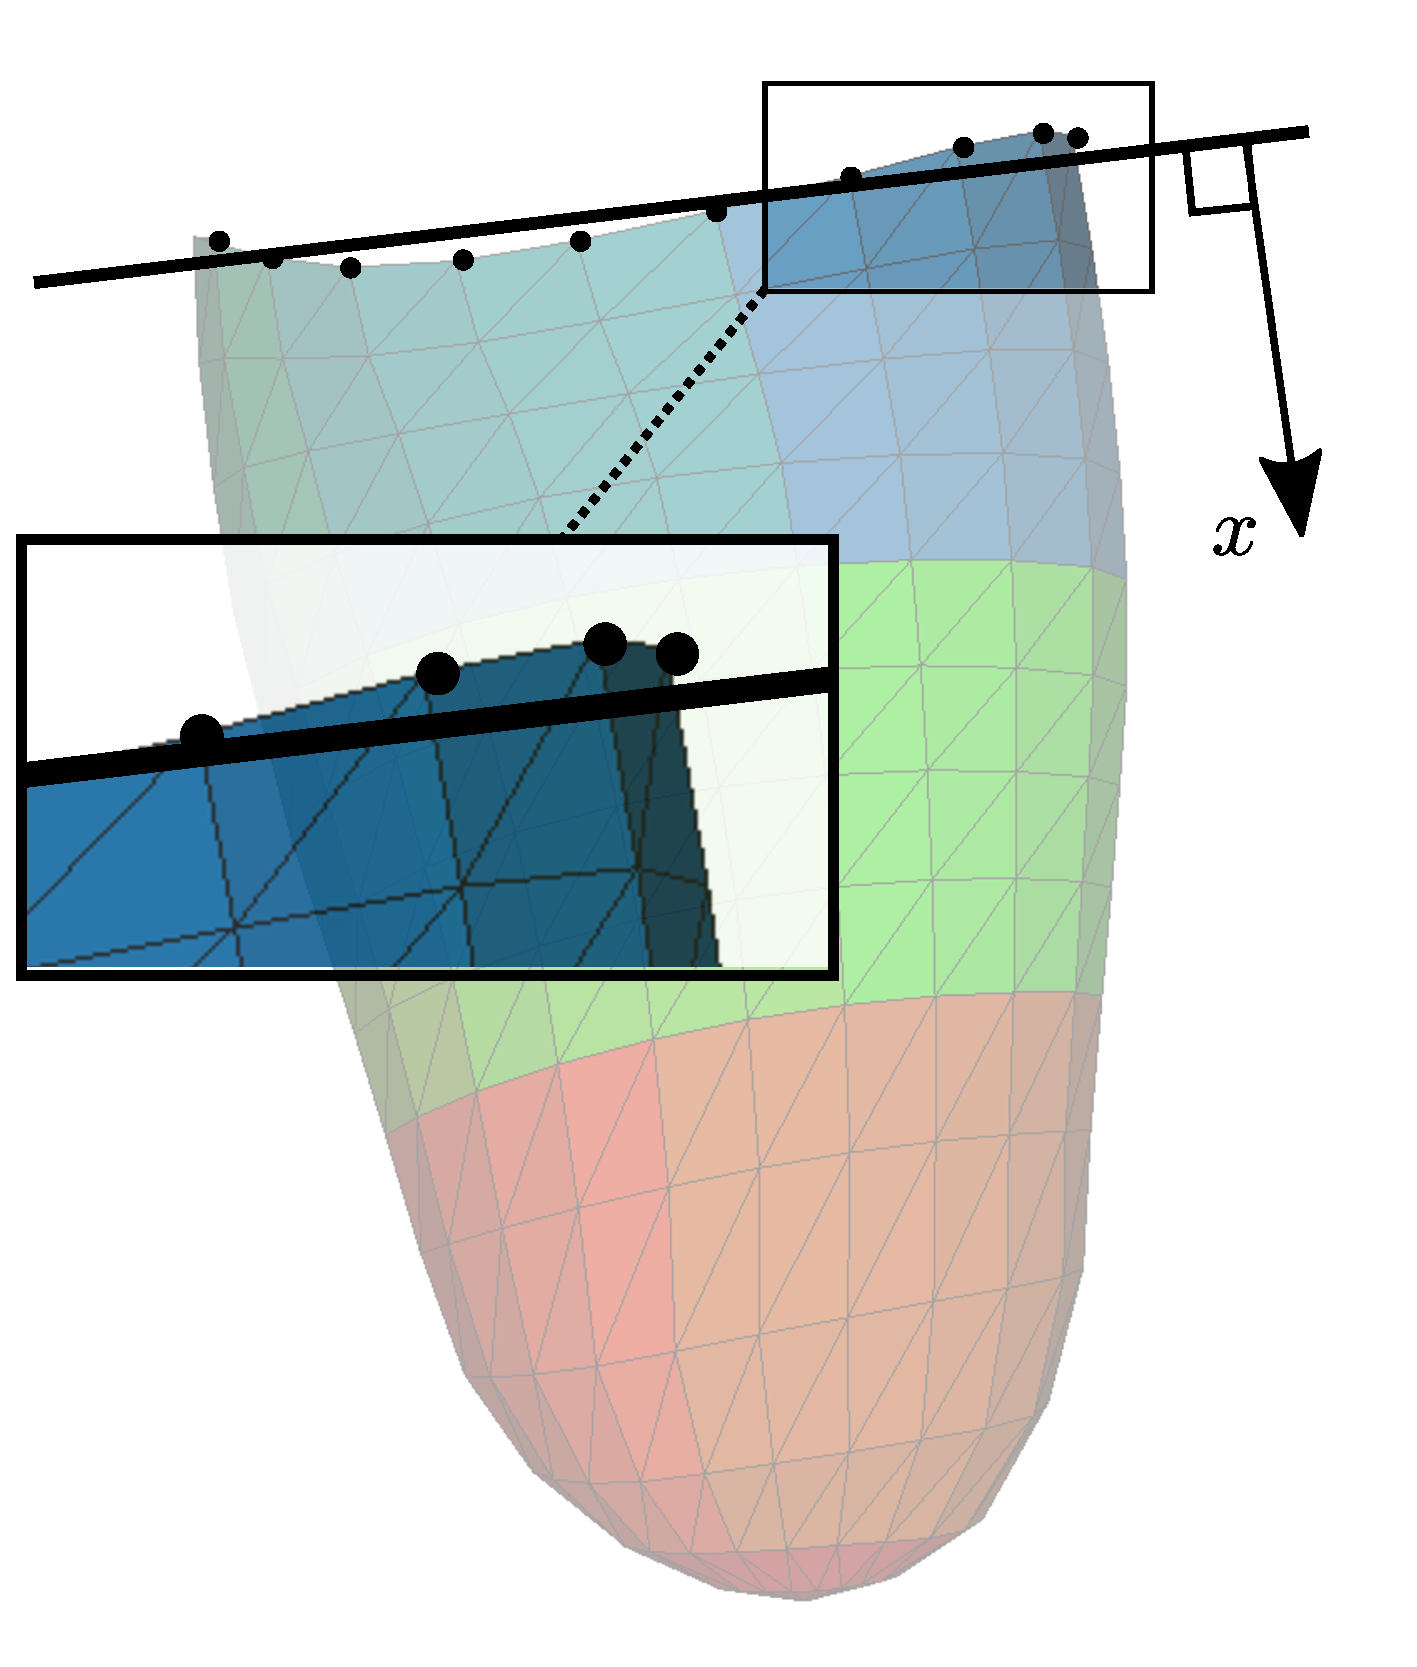
\includegraphics[width=\textwidth]{chapters/introduction/figures/geometry/strain_mesh_plane.pdf}
    \caption{\label{fig:strain_mesh_plane}}
  \end{subfigure}
  \begin{subfigure}[t]{0.36\textwidth}
    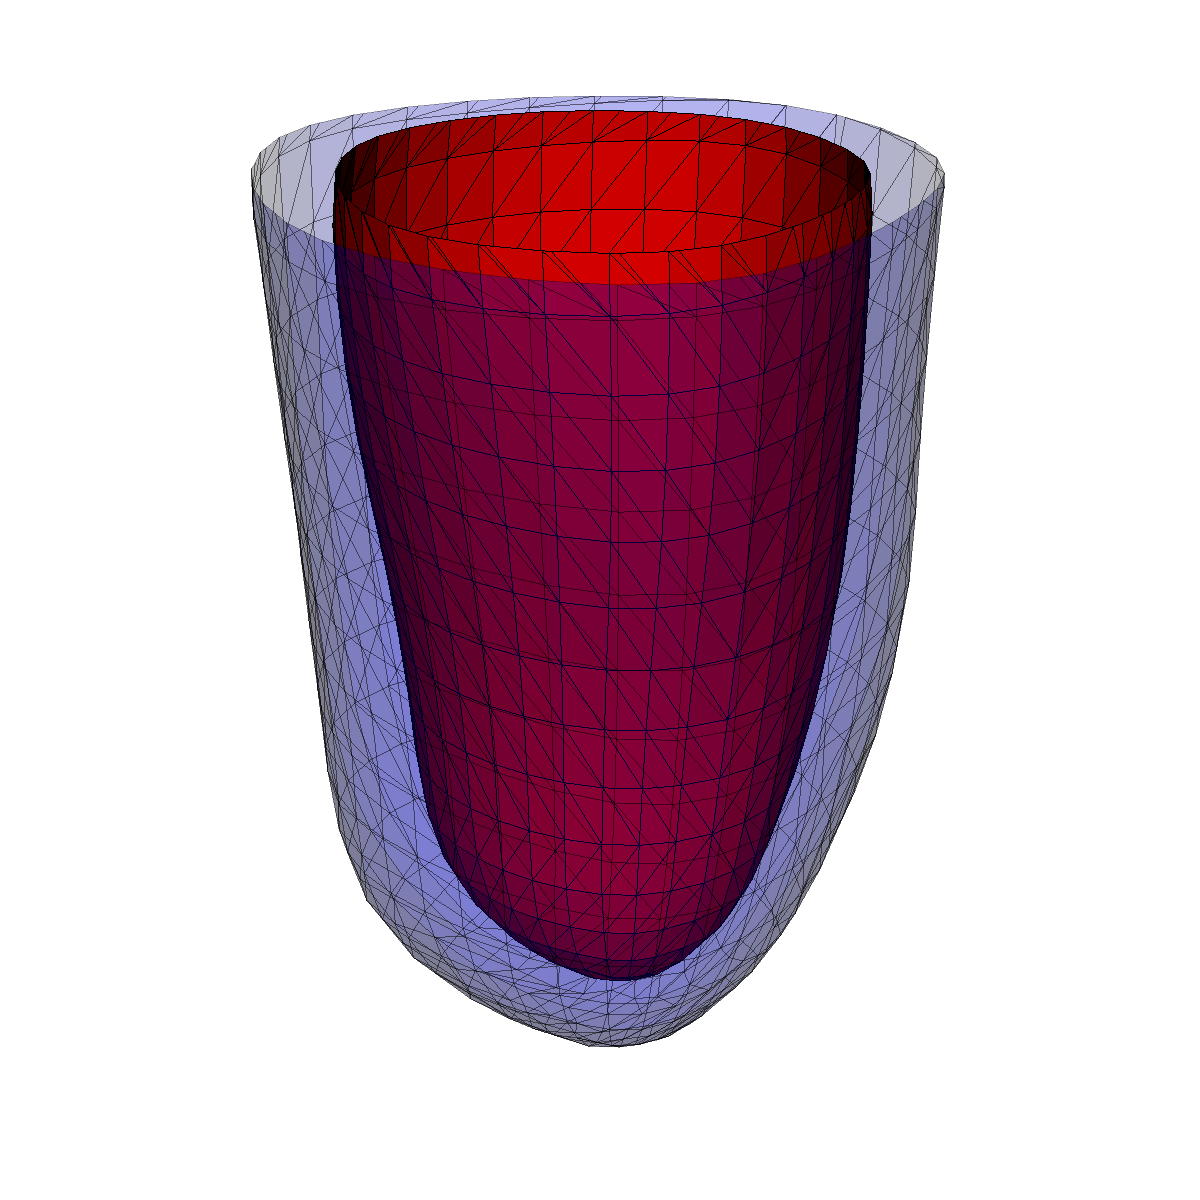
\includegraphics[width=\textwidth]{chapters/introduction/figures/geometry/cut.png}
    \caption{\label{fig:cut_intro}}
  \end{subfigure}
  \begin{subfigure}[t]{0.32\textwidth}
    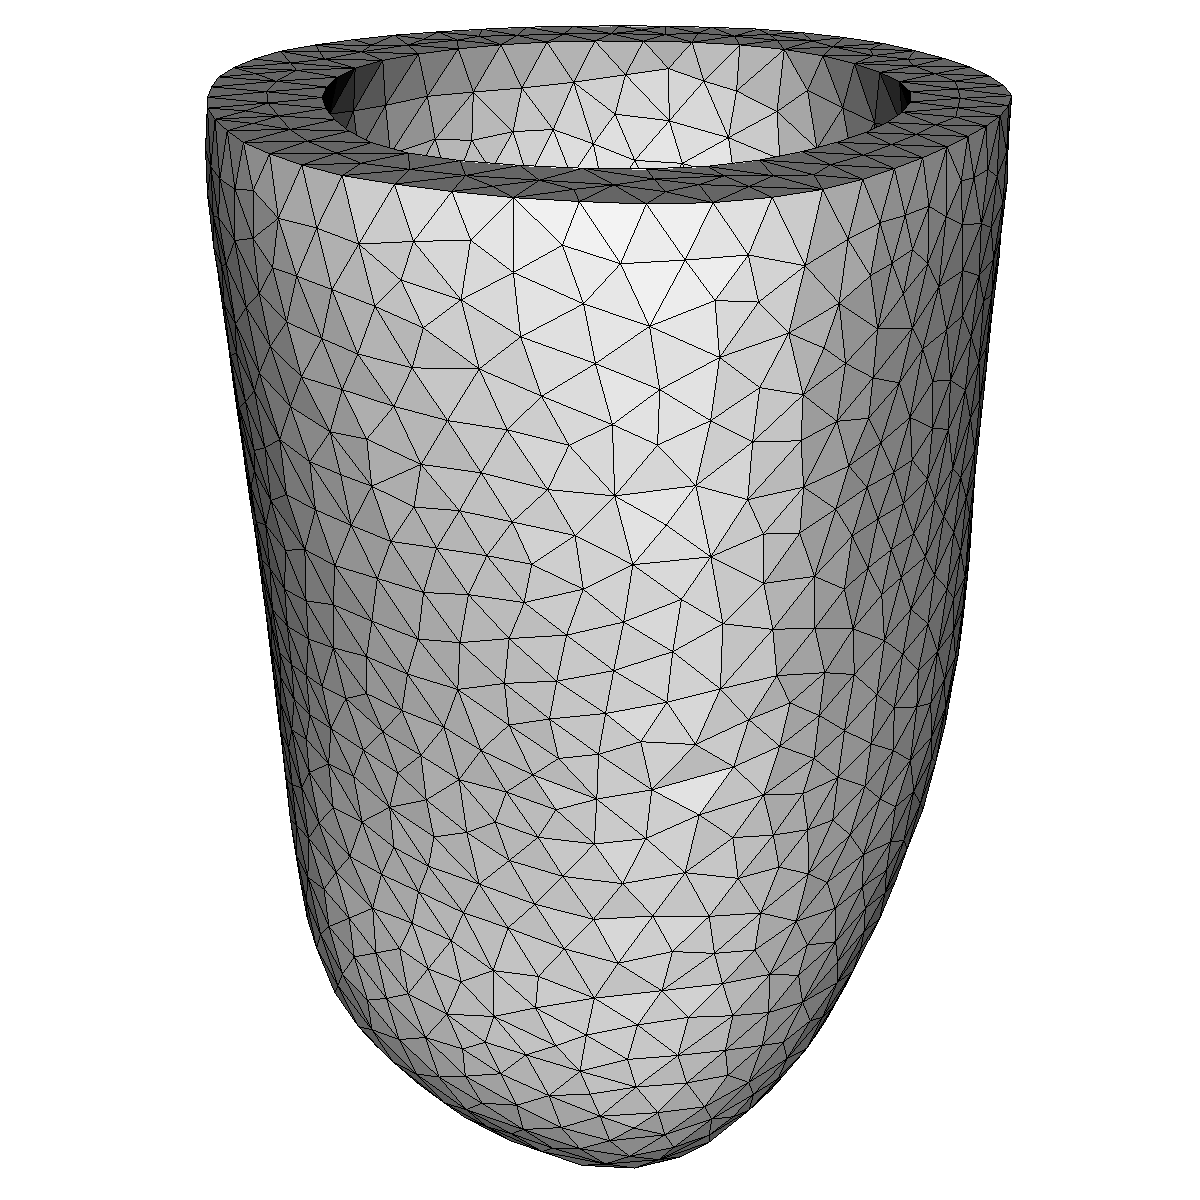
\includegraphics[width=\textwidth]{chapters/introduction/figures/geometry/mesh.png}
    \caption{\label{fig:mesh_intro}}
  \end{subfigure}
\caption{A least square fitting plane is fitted to the points
  belonging to the basal boundary in the strain mesh (Figure
  \ref{fig:strain_mesh_plane}). This plane is used to cut the endo- and
  epicardial surfaces (Figure \ref{fig:cut_intro}) and Gmsh is used to mesh
  these surfaces together (Figure \ref{fig:mesh_intro}). }
\label{fig:mesh_generation_intro}
\end{figure}



The actualy mesh generation is performed using Gmsh
\cite{geuzaine2009gmsh}, which meshes the endocardial and epicardial
surface togther unsing frontal-Delaunay meshing algorithm. Gmsh also marks
the endocardal, the epicardial  and the basal facets, along with the
endocardial and epicardial basal rings. 

% \begin{figure}[htbp]
%   \centering
  
%   \begin{subfigure}[t]{0.45\textwidth}
%     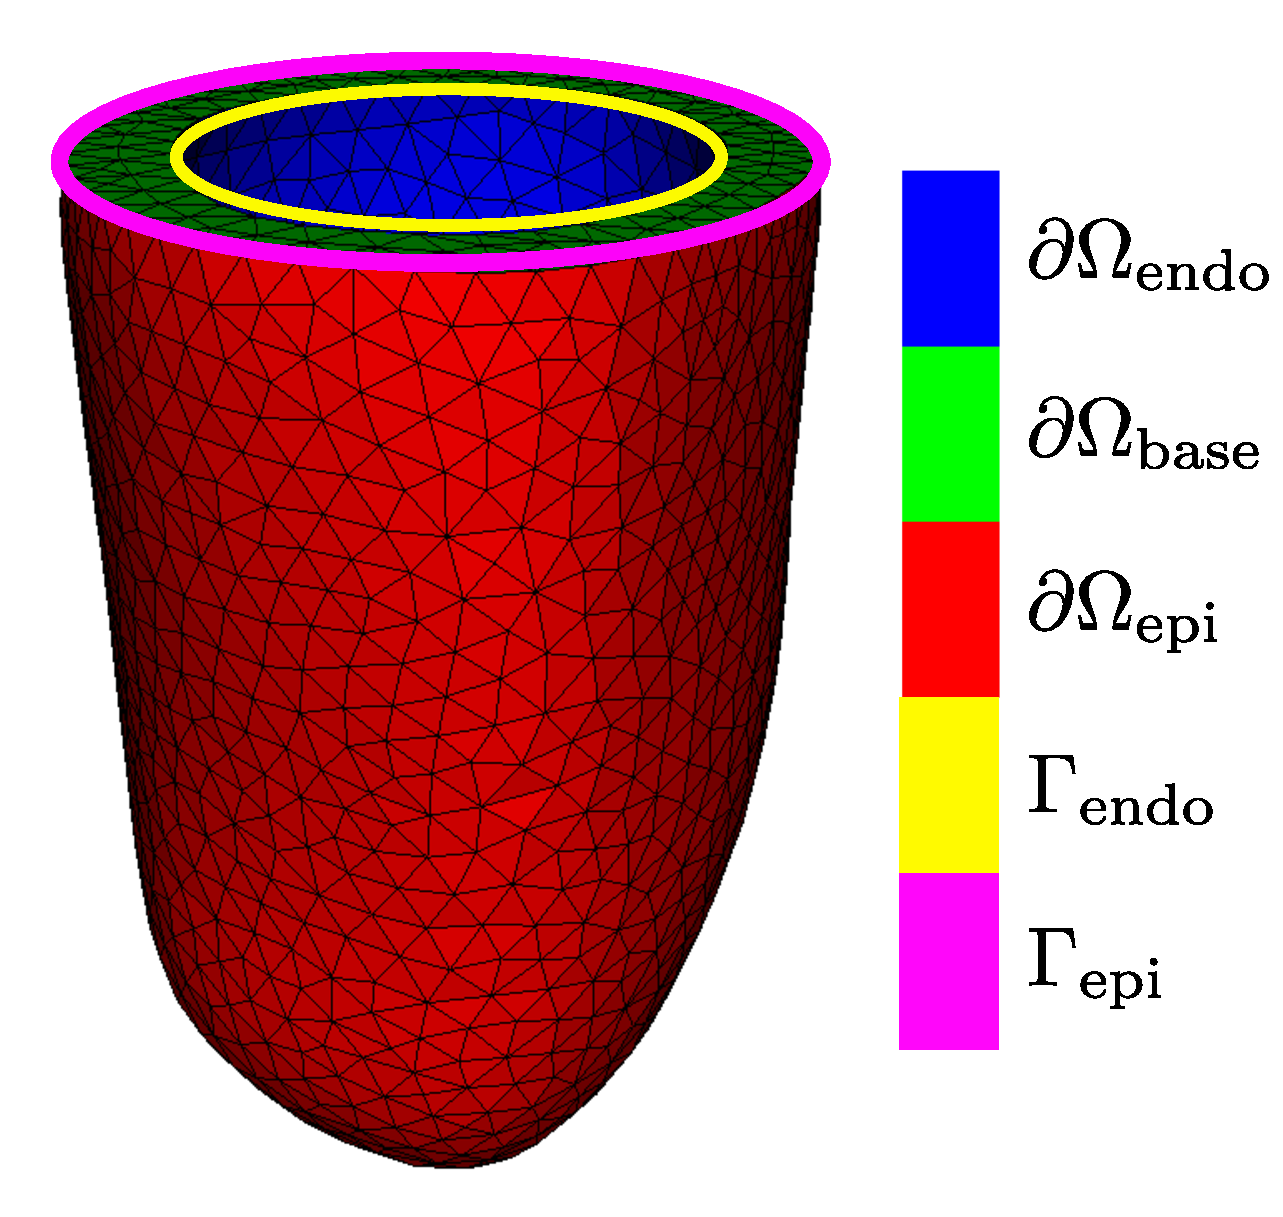
\includegraphics[width=\textwidth]{chapters/introduction/figures/geometry/markers_full.pdf}
%     \caption{\label{fig:markers_full}}
%   \end{subfigure}
% \caption{}
% \label{fig:echopac_output}
% \end{figure}



\begin{remark}
  The cavity volume is computed by generating the whole mesh, and the
  compute the volume using Equation \eqref{eq:volume_operator}. The cut size is
  found by using a one dimensional optimization algorithm with
  the objective funcitonal representing the squared error between
  computed and measured volume.
\end{remark}




\subsubsection{Rule-based fiber architecture}
\label{sec:rule_based_fiber}
Both the passive and active properties of the myocardium depends on
the underlying muscle fiber architecture, and it is therefore of high
relevance to capture this architecture as accuratley as
possible. Unfortunately, imaging technology does not currently provide a
way of extracting patients-specific fiber ortiention \emph{in
  vivo}. Diffusion Tensor Imaging (DTI) can be utilized to reconstruct
the fiber and lamiar structure \cite{rohmer2007reconstruction}
\emph{ex vivo}.

An alternative method for assigning myocardial fiber orientation is by
rule-based methods \cite{potse2006comparison, bayer2012novel}. 
In this thesis we have used an algorithm called the Laplace–Dirichlet
Rule-Based (LDRB) algorithm, proposed by Bayer et al \cite{bayer2012novel}.


\begin{figure}[htbp]
  \centering
  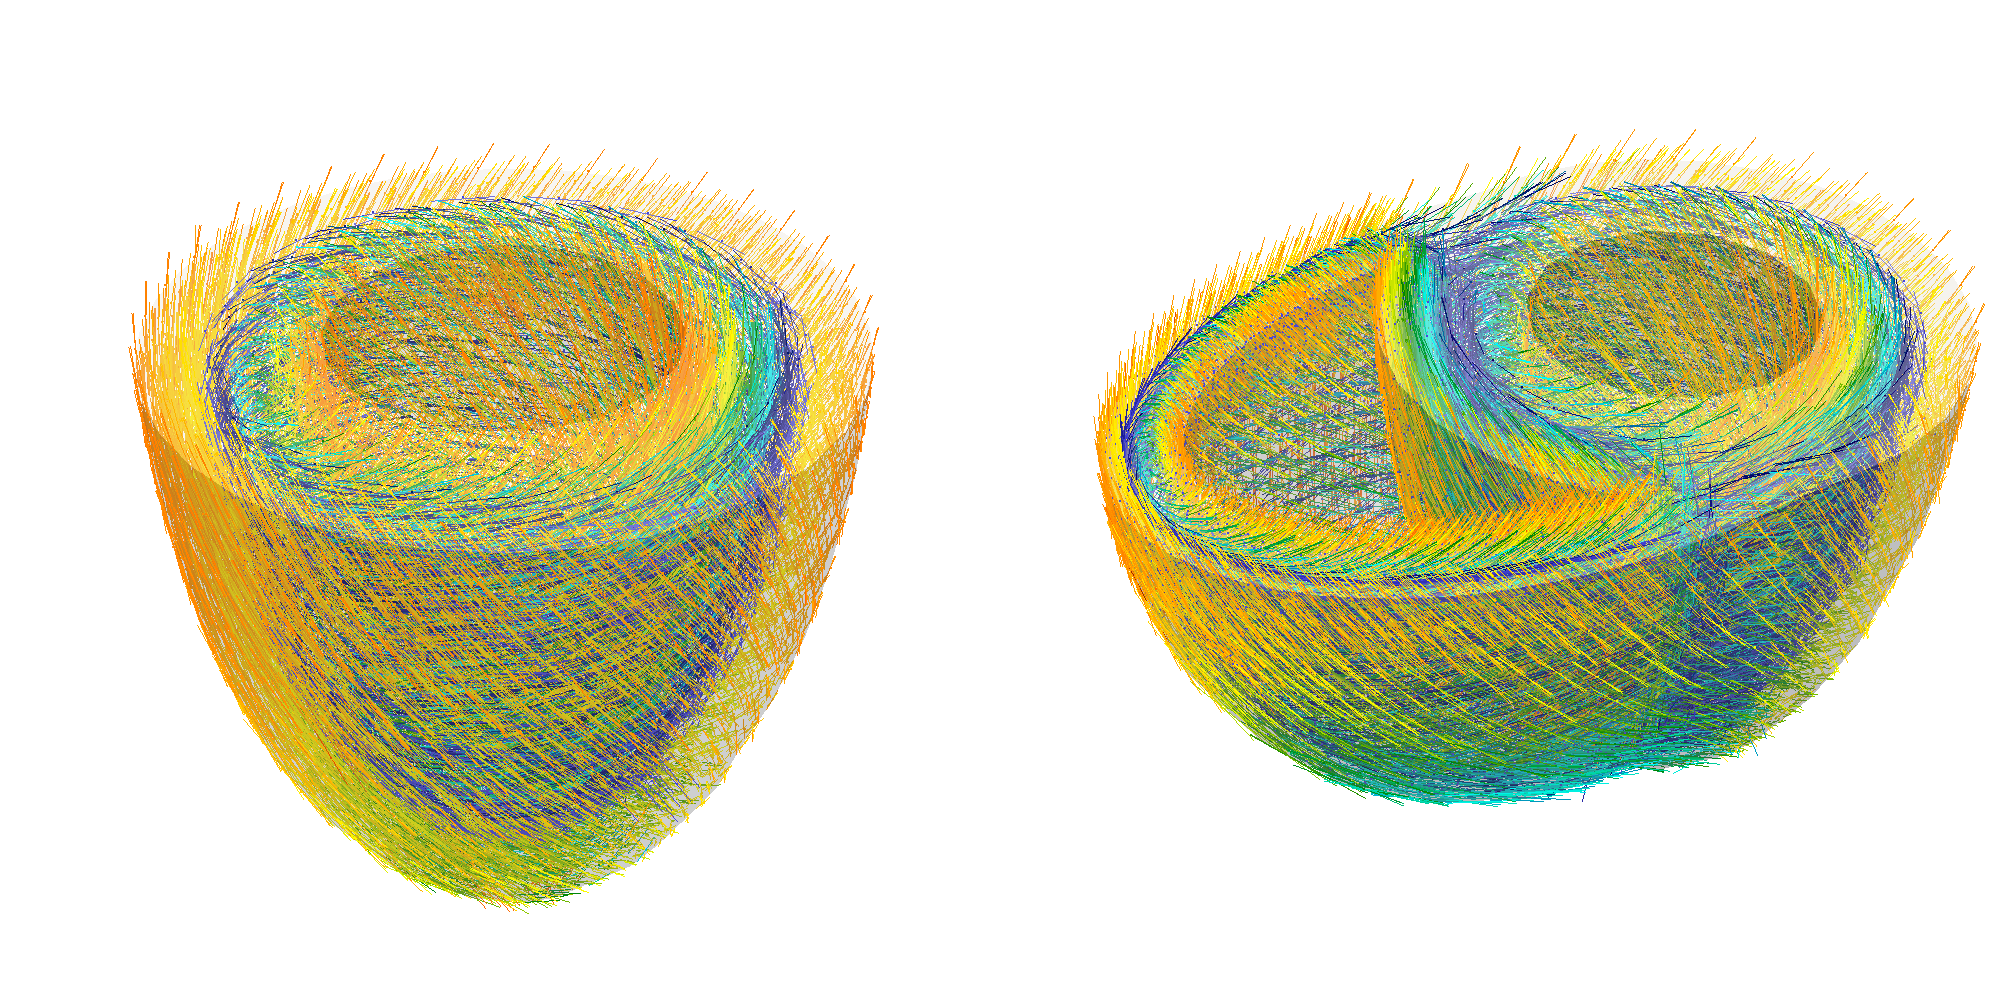
\includegraphics[width=\textwidth]
  {chapters/introduction/figures/fiber/fiber}
\caption{The LDRB algorithm \cite{bayer2012novel} applied to an LV
  (left) and BiV (right) geometry with an helix fiber angle of
  $60^{\circ}$ and $-60^{\circ}$ on the endo- and epicardium
  respectively. Color represents the helical angle, with blue being
  $0^{\circ}$ (circumferential) which can be seen in the midwall. }
\label{fig:echopac_output}
\end{figure}


The LDRB algorithm takes as
input the geometry $\Omega$, the helical fiber angle on the endo- and
epicardium ($\alpha_{\mathrm{endo}}$ and $\alpha_{\mathrm{epi}}$) and
the transverse fiber angle on the endo- and epicardium
($\beta_{\mathrm{endo}}$ and $\beta_{\mathrm{epi}}$), and outputs a
set of three orthogonal vector fields, one representing the fiber
angle $(\ef)$, one representing the sheet angle $(\es)$ and the final
diraciton is called the sheet normal direction $(\en)$

\subsubsection{The ventricular coordinate system}

When dealing with geometric shapes such as a left ventricle, finding a
coordinate system that is easy to work with is important. For
example, when studing spherical shapes, the spherical coordinate system is
usually easier to work with. Likewise, a coordinate system that is
easy to use when studying ellipsoidal shapes like the left ventricle is
the \emph{prolate spheroidal coordinate system} \cite{hunter1996kd}. 
The cartesian coordinates $(x,y,z)$ are related to the prolate
spheroidal coordinates by

\begin{align}
  \begin{split}
    x &= a \sinh \mu \sin \nu \cos \theta  \\
    y &= a \sinh \mu \sin \nu \sin \theta  \\
    z &= a \cosh \mu \cos \nu,
  \end{split}
\end{align}
where $a$ is the focal point, $\nu \in [0, \pi]$ is the longitudinal
coordinate, $\theta \in [0, 2\pi]$ is the azimuthal angle and $\mu$
is the radial coordinate. For an ellipse given by the equation
$\frac{x^2}{b^2} +\frac{y^2}{c^2}  = 1$ with $b$ being the semimajor
axis, and $c$ the semiminor axis, the focal point is given by
\begin{align}
  a =\sqrt{b^2 - c^2}.
  \label{eq:focal_point}
\end{align}
The prolate spheroidal coordinate axes are illustrated in
Figure~\ref{fig:prolate_coord}. There inverse relation, going from the
cartesian coordinate $(x,y,z)$ to the prolate spheroidal coordinate
$(\mu, \nu, \theta)$ given the focal point $a$ is a bit more
intricate, but can be computed as follows 
\begin{align}
  \begin{split}
    \nu &= \arccos (\tau) \\
    \mu &= \arccosh (\sigma) \\
    \theta &= \arctan \frac{z}{y} \\
    \tau &= \frac{1}{2a} \big( \sqrt{(x + a)^2 + y^2 + z^2} \\
    & \quad + \sqrt{(x - a)^2 + y^2 + z^2} \big) \\
    \sigma &= \frac{1}{2a} \big( \sqrt{(x + a)^2 + y^2 + z^2}\\
    & \quad - \sqrt{(x - a)^2 + y^2 + z^2}\big) 
  \end{split}
\end{align}
It is possible to estimate the focal point by taking $b$ in
\eqref{eq:focal_point} to be the maximum distance from the base to the
apex, and $c$ the maximum radius at the base. Using this estimate,
the base is assumed to be located approximately at the center of the
ellipsoid, i.e $\nu = \pi / 2$ \cite{land2015verification}.
% Compared to geometries used in
% benchmarking of cardiac mechanics problems, this is not a totally
% wrong assumption 
\begin{figure}[htbp]
  \centering
  \begin{subfigure}[t]{0.4\textwidth}
    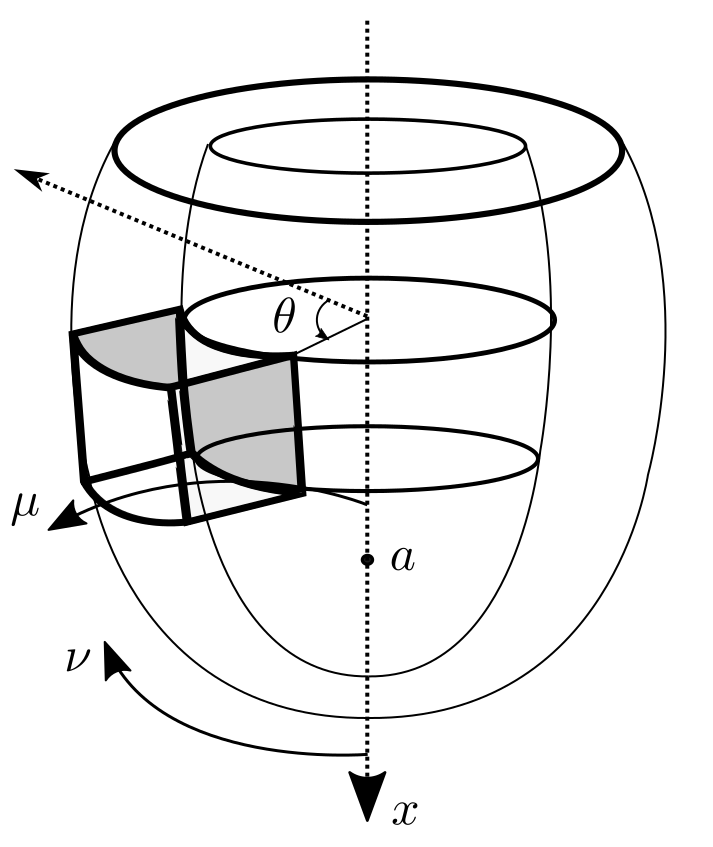
\includegraphics[width=\textwidth]{chapters/introduction/figures/geometry/prolate.png}
    \caption{\label{fig:prolate_coord}}
  \end{subfigure}
  \begin{subfigure}[t]{0.45\textwidth}
    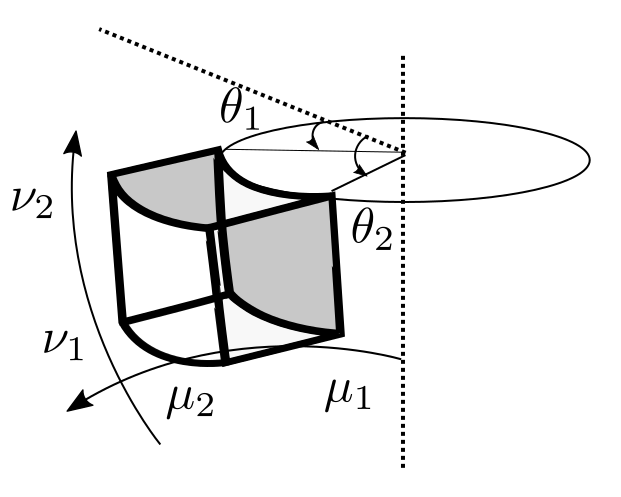
\includegraphics[width=\textwidth]{chapters/introduction/figures/geometry/prolate_cube.png}
    \caption{\label{fig:prolate_cube}}
  \end{subfigure}
\caption{}
\label{fig:prolate}
\end{figure}

This coordinate system can be used when e.g marking the mesh according
to the AHA segments

\subsection{Choosing the reference geometry}
\label{sef:reference_geometry}
The choice of reference geometry ..
 choosing the geometry with the smallest
volume as the reference geometry (i.e the end-systolic geometry)
(references), the mid-diastolic or the end-diastolic ??


A general problem in the biomechanics is that the geometry extracted from
imaging data is not the stress-free geometry, meaning the the geometry
that we observe is subjected to a physical load, e.g blood pressure.
This is analogous to finding the geometry of a deflated balloon, given
an image of and inflated one. Having this picture in mind, it is
intuitive that such a geometry not necessarily is unique.
Several techniques have been applied in order to obtain the unloaded
geometry, such as the inverse design analysis (ID)
\cite{govindjee1996computational} or the modified updated Lagrangian
formulation (MULF) \cite{gee2010computational}. Another popular
technique is a fixed point iteration scheme,  known as the
backward displacement method \cite{bols2013computational}. We briefly
explain the steps in this methods.

\begin{figure}[htbp]
  \centering
    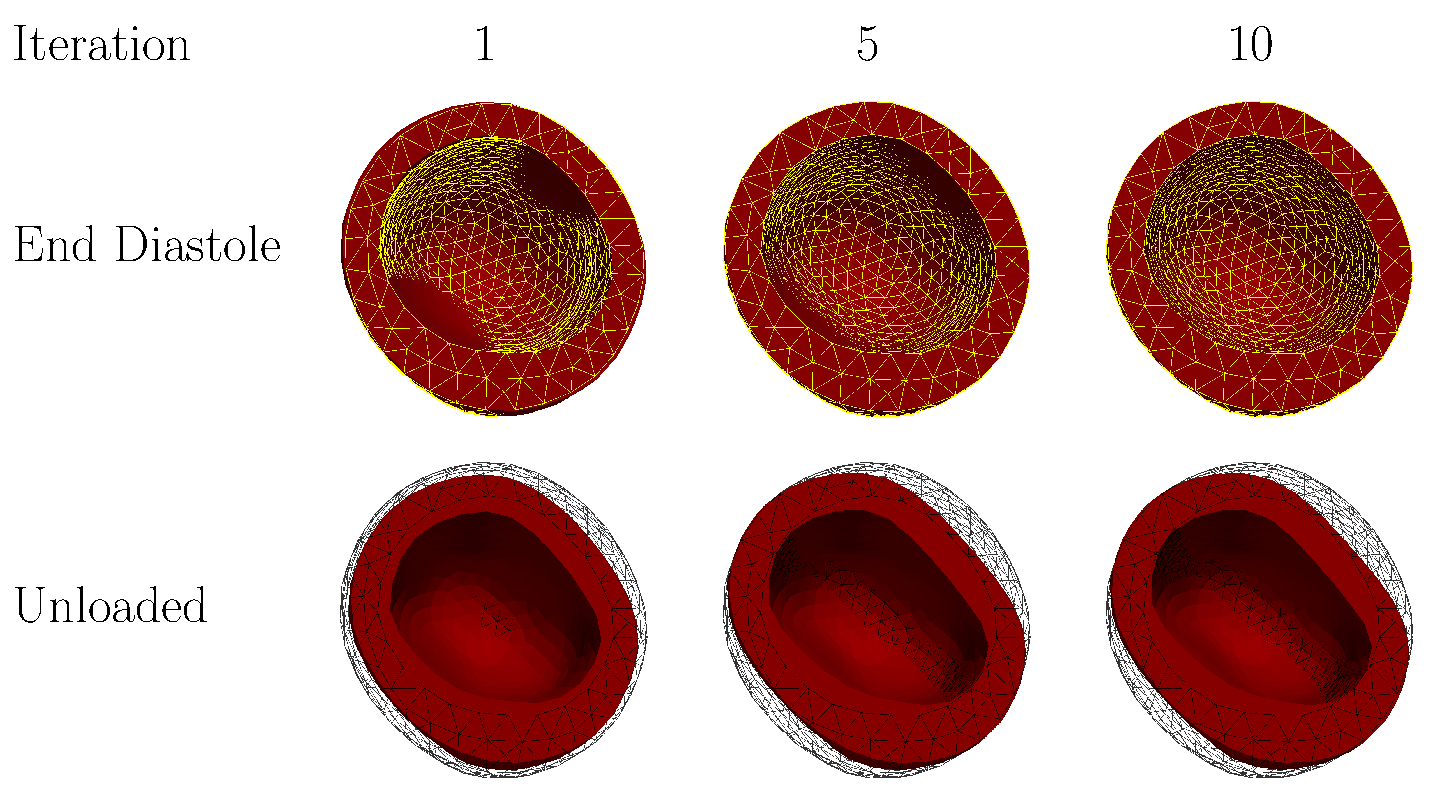
\includegraphics[width=0.9\textwidth]{chapters/introduction/figures/unloading/canvas.pdf}
\caption{Showing 1, 5, and 10 iterations of the backward displacement
  method applied to a left ventricular geometry. To row top shows the
  original geometry in solid and the inflated unloaded geometry in
  yellow wire-frame for 1,5 and 10 iterations. Bottom row shows the
  unloaded geometry in solid and the original image based geometry in wire-frame.}
\label{fig:unloading_lv}
\end{figure}


Suppose you are given geometry $\Omega_{\mathcal{I}}$ taken from some medical image, and
is thus loaded with some loads $\mathbf{T}$, and we want to find the unloaded geometry
$\Omega_{\mathcal{U}}$, which is so that when we load $\Omega_{\mathcal{U}}$ with $\mathbf{T}$,
you get back the starting geometry $\Omega_{\mathcal{I}}$. Let
$\Xvec_{\mathcal{I}}$ denote the coordinates in $\Omega_{\mathcal{I}}$, and
let $\mathbf{d}$ denote the displacement field which is the solution
of \eqref{some_force_balance_eq} with $\mathbf{T}$ representing
the traction on the endocardium, and which depends on the reference
coordinates. What we want, is to find
$\Xvec_{\mathcal{U}}$ so that $\Xvec_{\mathcal{I}} =
\Xvec_{\mathcal{U}} + \mathbf{d}(\Xvec_{\mathcal{U}})$. To
find  $\Xvec_{\mathcal{U}}$ we let
\begin{align}
  \Xvec_{n+1} = g(\Xvec_n) =  \Xvec_{\mathcal{I}} - \mathbf{d}(\Xvec_n),
  && \Xvec_0 = \Xvec_{\mathcal{I}}.
\end{align}
According to Banach Fixed Point Theorem, the mapping $g$ has a
fixed-point if $\| \nabla g \|_{\infty} = \| \nabla \mathbf{d}
\|_{\infty} < 1$. This means that as long as the deformation
resulting from the load $\mathbf{T}$ do not result in a stretch that
is more than $100 \%$, this method will converge. Of course the
question about convergence of the fixed point method is one
thing. Another thing is the convergence of the nonlinear solver.
For bi-ventricular geometries, the backward displacement method might
fail to converge especially if the tissue is soft and the pressure in
the right ventricle is large. In this case it can happen that the
right ventricle free wall collided with the septal wall when
subtracting the displacement. An example of this is illustrated in
Figure~\ref{fig:unloading_fail}. 

An alternative to the backward displacement method that do not
necessary converge towards a fixed point but provides an a more stable
way of obtainind an unloaded configuration was proposed in Ragahavan
et. al \cite{raghavan2006non}. Let $k$ be a scalar, and suppose we can write
\begin{align}
  \Xvec_{\mathcal{I}} = \Xvec_{\mathcal{U}} + k \cdot \mathbf{d}(\Xvec_{\mathcal{U}}).
\end{align}
Of course this assumption might not be true, but we can find a value of
$k$ that minimizes some residual using a 1D optimization
algorithm. Note that choosing $k = 1$, would be the same as applying
one iteration of the backward displacement method.

Since the backward displcement method really does converge towards a
fixed point, it is favorable to the Rahavan method. Therefore, a
hybrid approach is to apply the backward displacement method as
long as the non-linear solver converge, and switch to the Rahavan
method upon divergence.

\begin{figure}[htbp]
  \centering
    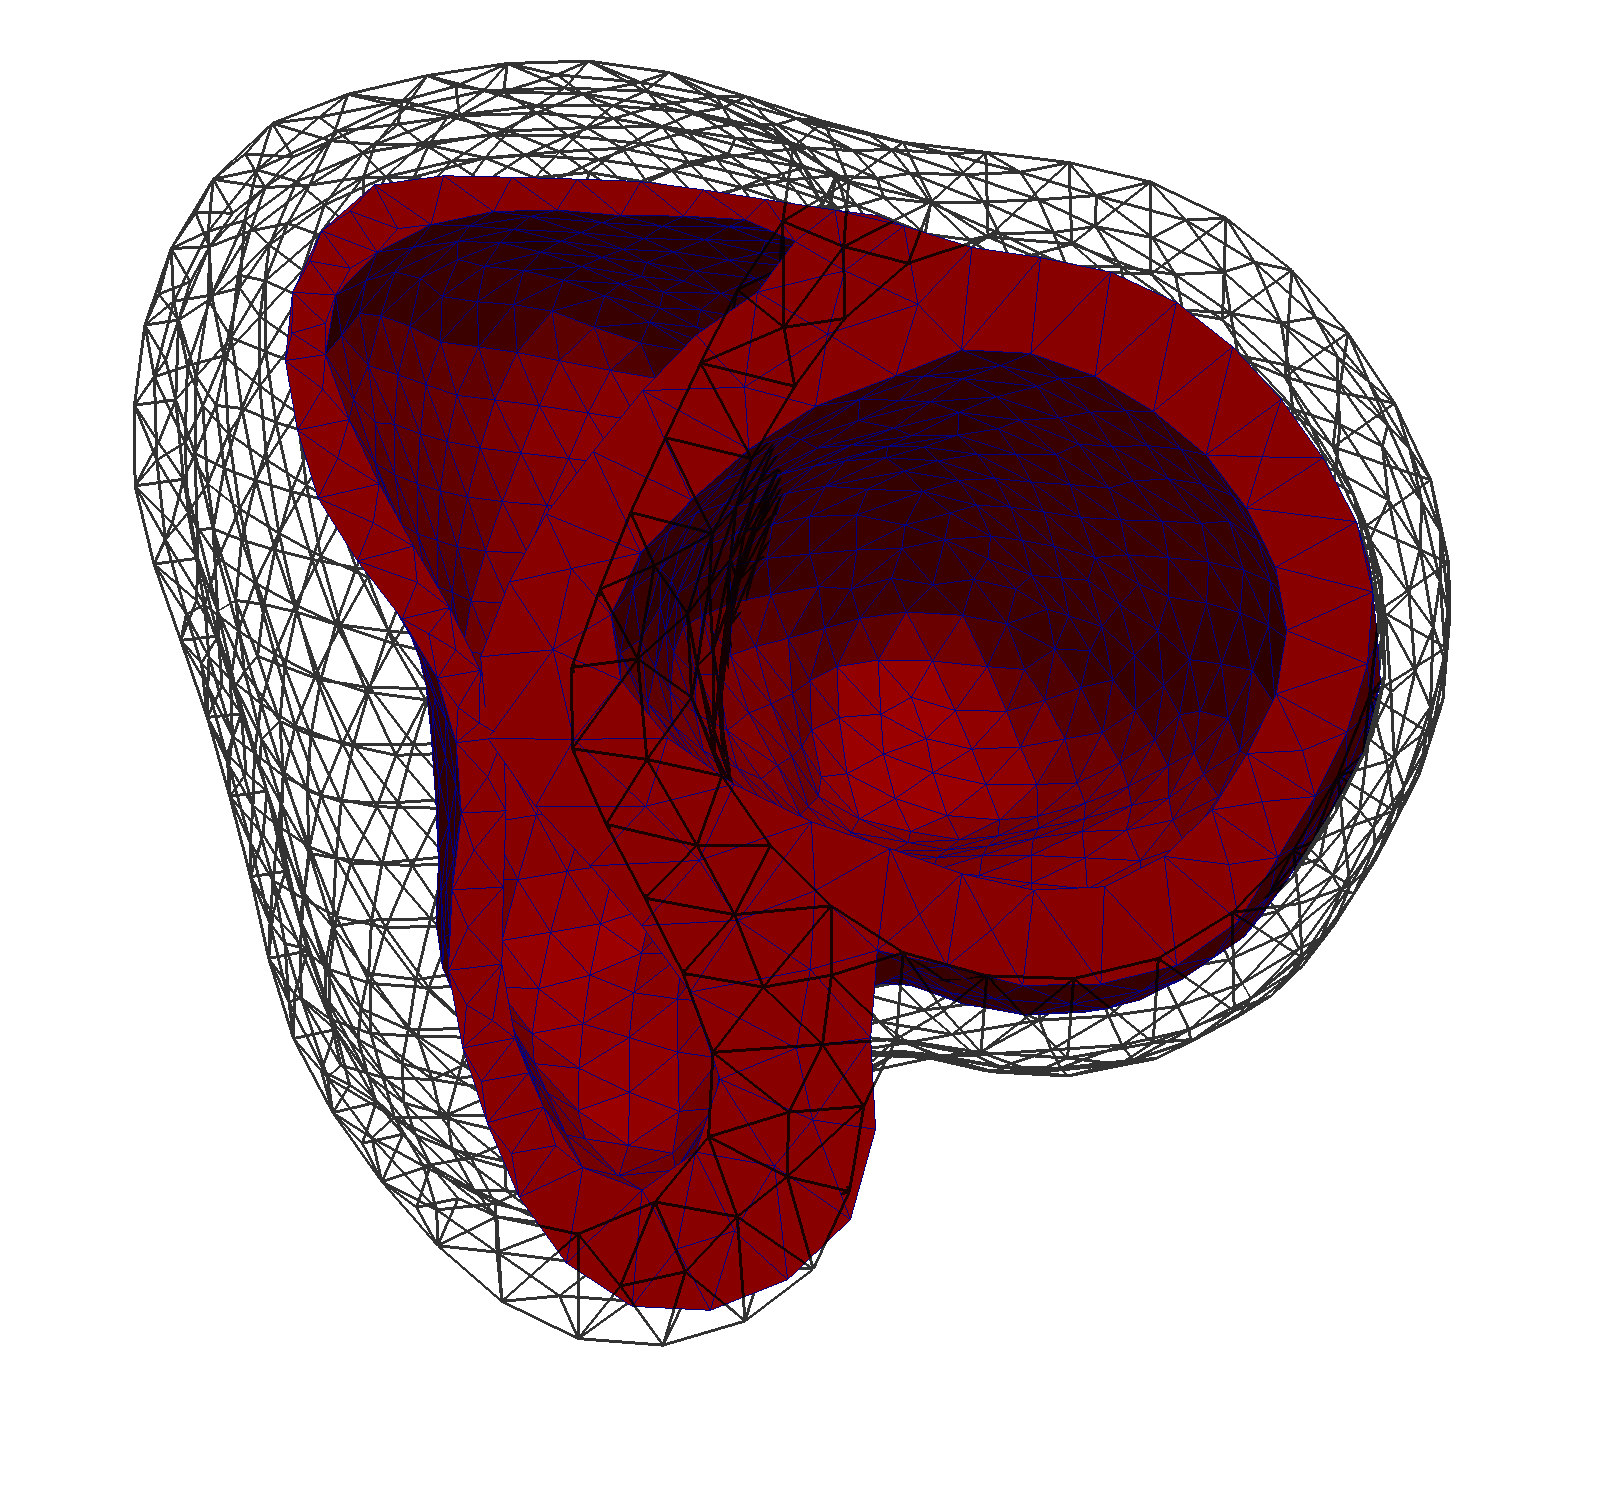
\includegraphics[width=0.5\textwidth]{chapters/introduction/figures/unloading_fail/unloading_fail.png}
\caption{Backward displacement method might fail for bi-ventricular
  geometries. This can be seen be noticing that the RV free wall is
  buckling and colliding with the septum.}
\label{fig:unloading_fail}
\end{figure}


For a transversely isotropic material (or orthotropic), the change in
fiber field when going from one geometry to another, has to be
considered. The natural thing to do is apply a \emph{Piola
  transformation} to the fibers in the image based geometry: Let
$\F_{n}= \I - \Grad \left(\mathbf{d}(\Xvec_n) \right)$ and left
$\ef^{n} = J^{-1}\F_{n} \ef$ where $\ef$ is the fiber field on
$\Omega_{\mathcal{I}}$. Another way is to regenerate the fibers (see
Section \ref{sec:rule_based_fiber}) using the new unloaded geometry as
input. We will see in the following numerical experiment that non of
these methods gives the desired result.









% \begin{remark}
%   The author has observed that when applying the backward
%   displacement method to bi-ventricular geometries subjected to a high
%   pressure in the right ventricle, and/or a thin RV free wall, then
%   the right ventricular free wall will in some cases collide with the
%   septum. Figure \ref{fig:unloading_fail} shows an example of
%   phenomena. In these cases a more robust approach (but less accurate)
%   is let $\Xvec_{n+1} = \Xvec_{\mathcal{I}} - k \mathbf{d}(\Xvec_n)$,
%   where $\Xvec_n$ is the results from the last converged fixed point
%   iteration, and use an optimization algorithm to determine the value
%   of $k$ than minimizes some residual. A similar approach has been
%   proposed in \cite{raghavan2006non}. 
% \end{remark}


\subsection{Data Assimilation}
The constitutive laws in cardiac mechanics comes from experiments
done on tissue slabs, and relates stresses in the material to strain.
If we had the same data available for a given patient we could easily
have performed a regression analysis in order to identify the
parameters in the contitutive model. However, this type of data
typically requires that tissue samples are taken from the myocardium,
which is not an option when dealing with living humans. In general,
when dealing with physical system such as the heart or weather
forecast it is not allways possible to design an experiment which
allows to determine all properties of a physical system
\cite{chapelle2013fundamental}. In such cases we have to take the
measurement that we have, and do our best to incorporate them into the
model. 

For example, the type of data that we usually have available, are data
that can be extracted using imaging techniques such as motion data,
volume traces, regional strain traces etc. One technique to estimate
model parameters based on such observations is called data assimilation.


The field of data assimilation has its roots in meteorology, where
a typical problem is to make predictions on the weather, based on
observations (of temperature, humidity etc.) at different locations. 


There are basically two main approaches to assimilate data;
\emph{sequential data assimilation} and \emph{variational data
  assimilation}. Sequential data assimilation, which is often
referred to as filtering, is based on a predictor-corector approach
where you start from your initial data and use a filter to predict the
next state. Once you have your measurement available you correct the
estimate based on the new observations. Some examples of sequential
procedures include Kalman filtering and Luenberger observers
\cite{chapelle2013fundamental}.

The other approach, called variational data assimilation, also known as
4D-var, is based on minimizing a cost functional that
represents the mismatch between observations and simulations, with
possibly additional regularization terms added to the objective
functional. We will focus this approach since this is the approach
that is taken in this thesis. For a more thourough review of other
methods we refer to \cite{chapelle2013fundamental}.


% The general setup for a variational data assimilation problem is the
% following.
\subsubsection{Pipeline}
\label{sec:data_assimilation_pipeline}

We will now explain the general setup and the main steps in variational data
assimilation. In order to keep consistent notation we will refer to
the \emph{state variable} as $\mathbf{w}$, which is our case
represents jointly the displacement and hydrostatic pressure
$\mathbf{w}=(\mathbf{u}, p)$.

The state varibles are described by some \emph{phyiscal forward
model} $\mathcal{M}$, which is our case is governed by the force balance
equation in \eqref{eq:force_balance_strong}. Moreover this model
typically depends on some parameters $\mu$ that we want to
adjust based on the observation at hand. For example, the unknown
parameters could be related to the stiffness of the myocardium which
which we want to adjust to each individual patient based on some
clinical obervations. We can therefore assume that the underlying
model can be written in the form $\mathcal{M}(\mathbf{w}, \mu) = 0$.

We are also given a set of measurements (or observations) that we want
to assimilate, and we denote a single observation by $y$.
For example, $y$ might by a volume measurements at some given time
points in the cardiac cycle, measuered using e.g unltrasound and image
processing techniques. The \emph{observation operator} $\mathcal{H}$,
is approximation of the observation and act as an operator from the
state space to the observation space. For a single obervation, we
therefore have the relation
\begin{align}
  y = \mathcal{H}(\mathbf{w}) + \xi, 
\end{align}
where $\xi = \xi_{\mathbf{\mathcal{H}}} + \xi_{\mathbf{y}}$ represents
both the error in the measurements ($\xi_{\mathbf{y}}$) (e.g
noise in the data) and error in the representation of the observation
($\xi_{\mathbf{\mathcal{H}}}$) (that $\mathcal{H}$ do not represent
the data good enough).

Finally all observations are combined into a single cost function
$\mathcal{J} = \mathcal{J}(\state, \mu)$ which represents the overall mismatch between
observations and simulations. The aim is to minimize this functional
while ensuring that the governing force balance equation is
satisfied. This can be done in the following steps

\begin{enumerate}
  \item For some initial guess $\mu_0$, solve the forward model
    $\mathcal{M} = 0$ to obtain $\state_0$.
  \item Compute $\mathcal{J}(\state_0, \mu_0)$.
  \item Compute the gradient $D \mathcal{J}(\state_0, \mu_0)$ to find
    the direction of the steepest descent.
  \item Move along the steepest direction and update the initial guess.
\end{enumerate}
The above steps are continued until we have reached a minimum for the
cost functional, e.g when the norm of the gradient becomes zero. In
practice we continue these steps until either the norm of the
gradient is below a certain tolerance or we have exceeded a maximum
number of iterations. Such a minimum may not allways exists, or there
may be several local minima. In the latter case, the choice of intial
guess determines which local minima you will end up in. The data
assimilation pipeline is summarized in
Figure~\ref{fig:data_assimilation}.

\begin{remark}
  There exists gradient-free optimization methods that can be used to
  avoid computing the gradient. Examples include genetic algorithms or
  particle swarm algorithms. The drawback with such methods is that
  they typically requires a lot of functional evaluations. In our
  case this is very computatinally exspensive, because every functional
  evaluation require us to solve the non-linear forward model. 
\end{remark}


\begin{figure}[htbp]
  \centering
    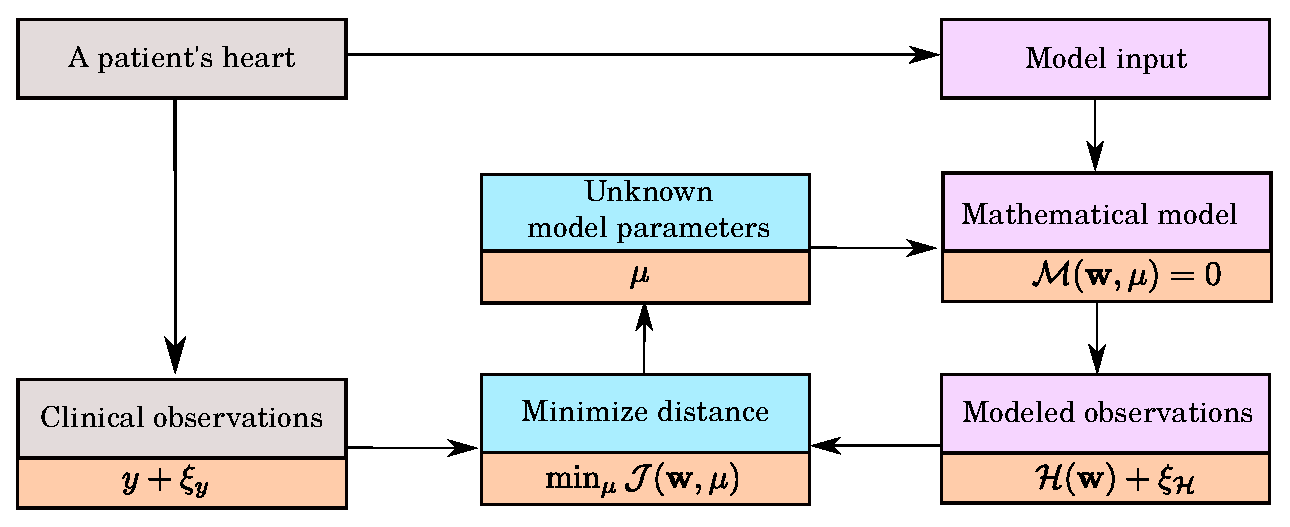
\includegraphics[width=\textwidth]{chapters/introduction/figures/data_assimilation.eps}
\caption{The different componenets involved in the data assimilation
  procedure. The mathematical description of each component is
  displayed below each box. From a patients heart we typicall extract information
  that are used as input to the model. This can for instance be
  information about geometry or information about boundary
  conditions. This model input is used to create a mathematical model
  of the heart, which also depends on some parameters $\mu$.
  These unknown parameters are determined by minimizing the distance
  between the clinical obervations $y$ and the modeled observation
  $\mathcal{H}(\mathbf{w})$.}
\label{fig:data_assimilation}
\end{figure}

We will now describe some of the main observation operators used in
this thesis before we explain how to solve the data assimilation
problem efficiently using the adjoint method. 


\paragraph{The volume observation operator
  $\mathcal{H}_{\mathrm{volume}}$}
In some cases, the ventricular cavity volume can easily be computed
analytically from the displacement field. Denote the inner cavity of
the left ventricle in the current configuration by
$\omega_{\mathrm{endo}}$. Further let $\mathrm{d} v$ and $\xvec$
denote an infinitesimal volume element and the coordinate in the
current configuration respectively. Then by the divergece theorem we have
\begin{align}
  \mathcal{H}_{\mathrm{volume}}(\uvec)= \int_{\omega_{\mathrm{endo}}} \mathrm{d} v =
  \frac{1}{3}\int_{\omega_{\mathrm{endo}}} \nabla \cdot \xvec \mathrm{d} v =
  \frac{1}{3}\int_{\partial \omega_{\mathrm{endo}}} \xvec \cdot \mathbf{n} \mathrm{d} s, 
\end{align}
where $\mathbf{n}$ and $\mathrm{d} s$ are the unit normal and a surface
element on the current configuration respectively.
Note that the boundary $\partial \omega_{\mathrm{endo}}$ includes the
endocardial basal boundary. However in the case when the base is flat
and fixed in longitudinal direction, the contribution from this
boundary integral will be zero. In this case the boundary integral
will be the same as the integral over the endocardial boundary, with
the only change being the change of sign on the normal vector. By
Nansens formula we obtain 
\begin{align}
  \mathcal{H}_{\mathrm{volume}}(\uvec)= -\frac{1}{3}\int_{\lvendo} \left( \Xvec + \uvec \right) J \F^{-T} \Nvec \mathrm{d}S,
  \label{eq:volume_operator}
\end{align}
where now $\lvendo$,  $\Xvec$, $\Nvec$ and $\mathrm{d}S$ are respectively the
endocardial surface, the referece coordinate, the unit normal and a
surface element in the reference configuration.


\paragraph{The strain observation operator
  $\mathcal{H}_{\mathrm{strain}}$}
Another observation that is encountered in this thesis is strain
measurements, or more precisely average regional strain in the
circumferential, radial or longitudinal direction. Let $\Omega_j$
denote the volume for which the strain should be averaged over, and
let $\mathbf{e}_k$ denote the unit vectorfield in the preferred strain
direction. Then for a given strain tensor $\mathbf{A}$ we define 
\begin{align}
  \mathcal{H}_{\mathrm{strain}}(\uvec) = \frac{1}{|\Omega_j|}\int_{\Omega_j} \mathbf{e}_k^T \mathbf{A}(\uvec) \mathbf{e}_k  \mathrm{d}V
\end{align}
The strain tensor $ \mathbf{A}$ is typically chosen to be the
Green-Lagrange strain tensor $\mathbf{E}$, or
the material displacement gradient tensor $\F - \I$.

\begin{remark}
  Measured strains are computed relative to some reference
  geometry, which do not always coinside with the reference geometry
  chosen for your simulation (for example if you use the unloaded geometry). In
  these cases you have to either recompute the measured strain
  according to the chosen referece for the simulation, or recompute
  the simulated strains according to the correct referece geometry for
  your measuments. In the latter case, one compute the strain tensor
  using the modified deformation gradient $\tilde{\F} = \F
  \F_{\mathrm{ref}}^{-1}$ where $\F_{\mathrm{ref}}$ is the deformation
  gradient from your current referece to the correct reference state. 
\end{remark}


\subsection{PDE-constrained optimization}


The variational data assimilation problem in cardiac mechanics belongs
to a class of problems called PDE-constrained optimization problems,
which can be formaluatd as follows:

\begin{equation}
  \begin{aligned}
    \label{eq:pde_constrained}
    & \underset{\mu \in P}{\text{minimize}}
    & &  \mathcal{J}(\state, \mu) \\
    & \text{subject to}
    & & \mathcal{M}(\state, \mu) = 0.
  \end{aligned}
\end{equation}

Here $\mathcal{J}(\state, \mu): W \times P \mapsto
\mathbb{R}$ is the objective functional that we want to minimize,
$W = V \times Q$ is the state space, $P$ is the parameter space
and $ \mathcal{M}(\state, \mu) = 0$ is the force balance
equation given by \eqref{eq:force_balance_strong}.



The typical way solving the problem \eqref{eq:pde_constrained} is to
turn the constrained problem into an unconstrained problem. One way
to do this is to consider the \emph{reduced functional}
\begin{align}
  \widehat{\mathcal{J}}(\mu) = \mathcal{J}(\state(\mu), \mu).
\end{align}
Since $\widehat{\mathcal{J}}$ is a pure function of $\mu$, we have
eliminated the constraint and turned the problem into an unconstrained
problem:
\begin{equation}
  \begin{aligned}
    \label{eq:pde_unconstrained}
    & \underset{\mu \in P}{\text{minimize}}
    & &  \widehat{\mathcal{J}}(\mu).
  \end{aligned}
\end{equation}

As discussed in Section \ref{sec:data_assimilation_pipeline}, a
solution to \eqref{eq:pde_unconstrained} satisfies the optimality
condition $D  \widehat{\mathcal{J}} = 0$. Here $D$ refers to the
total derivative with respect to the control $\mu$, while $D_{x}$
refers to the partial derivative with respect to $x$.

\subsubsection{Computing the funtional gradient} 
To move along the gradient descent it is required to actually
compute this functinal gradient. The ``naive'' approach would be to
estimate the gradient using finite difference approximation. However,
this require one functional evaluation for each degree of freedom in
the parameter space, so when the number of parameters are large this
becomes impractical.

By the chain rule we have
\begin{align*}
  D  \widehat{\mathcal{J}}  =  D  \mathcal{J}(\state(\mu), \mu) =
   D_{\mu}\mathcal{J}(\state(\mu), \mu) + D_{\state}\mathcal{J}(\state(\mu), \mu) D_{\mu}\state(\mu).
\end{align*}
The terms $D_{\state}\mathcal{J}(\state(\mu), \mu)$ and
$D_{\mu}\mathcal{J}(\state(\mu), \mu)$ are typically straight forward
to compute. The term $D_{\mu}\state(\mu)$, on the other hand, is more
involved to compute.  If the take the total derivative of the
force balance equation, we obtain
\begin{align*}
  D \mathcal{M}(\state(\mu), \mu) =
  D_{\state} \mathcal{M}(\state(\mu), \mu) D_{\mu}\state(\mu)
  +  D_{\mu} \mathcal{M}(\state(\mu), \mu)  = 0,
\end{align*}
and we see that
\begin{align}
  D_{\state} \mathcal{M}(\state(\mu), \mu)  D_{\mu}\state(\mu) = - D_{\mu} \mathcal{M}(\state(\mu), \mu).
  \label{eq:tangent_linear_model}
\end{align}
The system \eqref{eq:tangent_linear_model} is known as the tangent
linear system, and can be computed numerically using ordinary
algorithmic differentiation techniques. However it requires that you
first specify theparameter $\mu$, meaning that it becomes expensive to
compute the functional gradient at several control points. 

We could instead plug in the solution to
\eqref{eq:tangent_linear_model} to get
\begin{align}
   D  \widehat{\mathcal{J}}
    % &=  D_{\mu}\mathcal{J}(\state(\mu), \mu)
      % - D_{\state}\mathcal{J}(\state(\mu), \mu) \left(  D_{\state} \mathcal{M}(\state(\mu), \mu) \right)^{-1} D_{\mu} \mathcal{M}(\state(\mu), \mu) \\
      &= D_{\mu}\mathcal{J}(\state(\mu), \mu) - z^* D_{\mu} \mathcal{M}(\state(\mu), \mu),
        \label{eq:functional_gradient}
\end{align}
where
\begin{align*}
  z^* = D_{\state}\mathcal{J}(\state(\mu), \mu) \left(  D_{\state} \mathcal{M}(\state(\mu), \mu) \right)^{-1} \\ 
  \implies z^* D_{\state} \mathcal{M}(\state(\mu), \mu) =  D_{\state}\mathcal{J}(\state(\mu), \mu)
  \label{eq:adjoint_equation}
\end{align*}
Note that in \eqref{eq:functional_gradient}, the variable $z^*$
represents a Lagrange multiplier enforcing the PDE constraint.  
In order to solve this system we need to have on the form $A\xvec =
b$, and we take the adjoint (Hermitian transpose) to get
\begin{align}
  D_{\state} \mathcal{M}(\state(\mu), \mu)^* z = D_{\state}\mathcal{J}(\state(\mu), \mu)^*
\end{align}
Equation \eqref{eq:adjoint_equation} is called the adjoint equation.
To compute the gradient we can now solve for $z$ and then insert $z^*$
into \eqref{eq:functional_gradient} to compute the gradient.


% Now suppose we have discretized the partial differental equation
% $\delta \Pi(\state, \mu) = 0$, which reduces to a system of the form
% $\mathbf{A} \state = \mathbf{b}$, with possible all terms depending on
% the parameters $\mu$. The gradient of the cost functional with
% respect to the parameter is given by
% \begin{align}
% -  \frac{\mathrm{d} \mathcal{J}}{\mathrm{d} \mvec} = \frac{\partial \mathcal{J}}{\partial \mvec}
%   + \frac{\partial \mathcal{J}}{\partial \state} \frac{\mathrm{d} \state}{\mathrm{d} \mvec}.
%   \label{eq:grad_cost}
% \end{align}
% Here $\frac{\mathrm{d}}{\mathrm{d} \mvec}$ denotes the total
% derivative, while $ \frac{\partial}{\partial \mvec}$ denotes the
% partial derivative. Computing the partial derivatives in
% \eqref{eq:grad_cost} are usually straight forward, while computing  $
% \frac{\mathrm{d} \state}{\mathrm{d} \mvec}$ is hard. To see this, let
% us differentiate the equation $\mathbf{A} \state = \mathbf{b}$ with
% respect to $m_i$, and solve for the 


% \begin{remark}
  
%   In data assimilation we typically want to copmute the gradient of
%   the cost function because we want to employ gradient-based
%   optimization algorithms for finding the ``optimal'' parameter
%   set. In other cases, the gradient might be important because it
%   tells you something about the sensitivity of your function of
%   interest with respect to the parameters. For example, if you have a
%   model with many input parameters, you may want to identify what
%   impact the different parameters has on the output. Perturbing each
%   parameter and observing the chane in the objective function quickly
%   becomes infeasible when the number of parameters becomes large, in
%   which case the adjoint aproach offer a possible solution. 
% \end{remark}

\subsubsection{Dolfin-Adjoint}

Dolfin-Adjoint is a software package that based on the FEniCS project
which aims to derrive the discrete adjoint equation and the tangent
linear models of finite element models implemented within the FEniCS
framework. While the tradional approach is to derrive the adjoint code
from the forward code using automatic differentiation tools,
Dolfin-Adjoint utilises the high level symbolic representation
\cite{UFL} in FEniCS to derrive the discrete adjoint equations from
the discrete forward eqations, and then the FEniCS system derrives the
adjoint code from the discrete adjoint equations. 





\subsubsection{Regularization}
Regularization is an important concept in many scientific disiplines
concerned with data fitting. When using data that essentially are
realizations of a stochastic proccess, we need to take into account
that the data are corrupted with noise. Moreover, the model we are using
is a simplification of a phyiscal proccess, and fitting the
data exactly to the model is unrealistic. This is especially
important if the number of parameters we are trying to estimate are
more than the number of data points used as input. In such cases it is often
beneficial to make some assumptions about the solution we are looking
for in order to avoid overfitting. For example, we may assume that the
parameter we are searching for is smooth. Suppose that $\mu \in
H^1(\Omega)$ is the parameter we want to find, and that we want to
favor smooth solutions. Then the norm of the gradient $\| \nabla \mu
\|$ should be small. One way to achieve this is to add a penalty term
to the objective functional so that in stead of minimizing
$\mathcal{J}(\state, \mu)$ we minimize $\mathcal{J}(\state, \mu) +
\lambda \| \nabla \mu\|$, where the constant $\lambda$ controls the
amount of regularization and is called the regularization parameters.
Note that in the limit $\lambda \rightarrow \infty$ we would end up
with a constant function. This approach is referred to as Tikhonov
regularization.

Another reason for using regularization is to stabilize the solver for
the underlying PDE that we solve. Parameters with sharp spikes
can make Newtons iterations in-feasible, and restricting the
parameter space to exclude such solutions might help stabilize the
Newton solver. 


% \subsubsection{Solving the PDE-constrained optimization problem using the
%   adjoint method}

% Via Reduced functional

% We will now explain what we mean by ``adjoint-based'', and why this
% approach is a key ingredient. The main theory presented here is taken
% from the dolfin-adjoint web page. A word about dolfin adjoint...\ref{}


% In order to apply optimisation algorithm...
% We reduce the objective functional to be a function of the control
% parameters only, $\hat{I}(\mvec) := I(\state(\mvec), \mvec)$. Consider an
% initial value of the parmameters $\mvec = \mvec^0$. If $\hat{I}(m)$ is defined
% and differentible in a neighborhood of $\mvec^0$ then $\hat{I}$ (and
% consequently $I$) decreases fastest in the direction of the gradient, 
% \begin{align}
%   \nabla_{\mvec} \hat{I}(\mvec^0) = \begin{bmatrix}
%     \frac{\mathrm{d} \hat{I}(\mvec^0) }{\mathrm{d} m_1},
%     \frac{\mathrm{d} \hat{I}(\mvec^0) }{\mathrm{d} m_2},
%     \cdots
%     \frac{\mathrm{d} \hat{I}(\mvec^0) }{\mathrm{d} m_N}
%   \end{bmatrix}^T.
%   \label{eq:functional_gradient}
% \end{align}
% Here $\frac{\mathrm{d} \hat{I} }{\mathrm{d} m_i}$ represents the
% total derivative:
% \begin{align}
%   \frac{\mathrm{d} \hat{I} }{\mathrm{d} m_i} = \frac{\mathrm{d} I (\state(\mvec), \mvec))}{\mathrm{d} m_i} = \frac{\partial  I }{\partial \state} \frac{\mathrm{d} \state}{\mathrm{d} m_i} + \frac{\partial  I }{\partial m_i}.
%   \label{eq:functional_derivative_component}
% \end{align}
% In other words, the sequence
% \begin{align}
%   \mvec^{k+1} = \mvec^{k} - \gamma_k \nabla_{\mvec} \hat{I}(\mvec^k), \gamma_n \in \mathbb{R}
% \end{align}
% satisfies $\hat{I}(\mvec^{k+1}) \leq \hat{I}(\mvec^k) \; \forall k \geq
% 0$, and converges towards a local minimum. If $\hat{I}$ is convex then
% the minimum is also global.
% Being able to compute the gradient of the objective functional wrt to
% the control parameters allows us to employ gradient based optimization
% methods which are in general superior to gradient free methods.
% One way to compute the gradient is by means of the finite difference
% approach: For a given parameter $\mvec = \mvec^*$ we have
% \begin{align}
%   \frac{\mathrm{d} \hat{I} }{\mathrm{d} m_i}( \mvec^*) =
%   \lim_{h \mapsto 0} \frac{\hat{I}(\mvec^* + h\mathbf{e}_i) - \hat{I}(\mvec^*)}{h}, 
% \end{align}
% where $\mathbf{e}_i \in \mathbb{Q}$ is the $i$'th canonical basis
% vector. If $\dim(\mathbb{Q}) = N$, this approach would require $N+1$
% functional evaluations. Moreover, since the state-variables depends upon the
% control variables, we would also need to solve the force balance
% equation $N+1$ times, which is typically very copmutationally
% expensive. Hence, this approach is typically infeasable when the
% dimesion of your parameterspace is large. In this case the adjoint
% approach is much better. If $A$ is an operator (e.g a matrix), then
% the adjoint operator $B$ satisfies the relation $\langle Au, v \rangle
% = \langle u, Bv \rangle$, and we write $ B = A^*$. Here $(\cdot)^*$
% denotes the Hermitian transpose, which in the case where $A$ is a real
% matrix is just the transpose of $A$, $A^T$.  


% Note that the gradient in
% \eqref{eq:functional_gradient} can be rewritten (using the chain rule)
% as
% \begin{align}
%   \nabla_{\mvec} \hat{I} =  \frac{\partial  I }{\partial \state} \nabla_{\mvec} \state
%   + \frac{\partial  I }{\partial \mvec},
%   \label{eq:functional_gradient_chain}
% \end{align}
% in which the $\dim(\mathbb{V}) \times \dim(\mathbb{Q})$ matrix
% $\nabla_{\mvec} \state$ is difficult to compute.
% Differentiating the force-balance equation \ref{} with respect to the
% control parameters yields
% \begin{align}
%   & \nabla_{\mvec} \delta \Pi(\state, \mvec) = 0 \\
%   \implies & \frac{\partial  \Pi }{\partial \state} \nabla_{\mvec} \state
%   + \frac{\partial  \Pi }{\partial \mvec} = 0 \\
%   \implies & \nabla_{\mvec} \state =
%              - \left( \frac{\partial  \Pi }{\partial \state} \right)^{-1} \frac{\partial  \Pi }{\partial \mvec}.
% \end{align}
% Inserting this expression for $\nabla_{\mvec} \state$ into
% \eqref{eq:functional_gradient_chain}, gives
% \begin{align}
%   \nabla_{\mvec} \hat{I} =  - \frac{\partial  I }{\partial \state}
%   \left( \frac{\partial  \Pi }{\partial \state} \right)^{-1} \frac{\partial  \Pi }{\partial \mvec}
%   + \frac{\partial  I }{\partial \mvec}.
% \end{align}




\subsection{Identifiability of parameters}
% Try dividing heart mesh is different segment, discuss uniqueness of
% paraperers
% Discuss regularization technices
When dealing with parameter estimation, you should always consider
questions about identifiability and uniquness. This depends on the
model, the data and the objective functional
\cite{hadjicharalambous2015analysis}. A first test should be to
generate synthetic data with some prescribed parameters, feed this
error-free data to the data assimilation method, and ensure that you
are able to retrieve the parameters that generated that data. If you
end up with a different parameter set than the one generated the data,
your problem is not \emph{structuraly identifiable}
\cite{chabiniok2016multiphysics}. Your problem is said to be
\emph{practical identifiable} if the parameters can be determined
uniquely based on the data at hand. If the test passes you shold try
to add noise to the data, and see if your data assimilation is stable
with respect to noise in the measurement, and you should quantify the
model out error versus the model input error. Demonstrating identifiability is
often difficult, especially when your data is corrupted with noise,
and when the complexity of the model increases. Balancing the
complexity of model in terms of \emph{model fidelity}, i.e wheter your
model is rich enough to representing the data, and the identifiability
is often key in order to have robust model. A too simple model will
often fail to represent your data, while a too complex model, might
give completely differet answers with just a slight perturbation of
the data, i.e with noise added to the measurement. The same problem is
encountered in other scientific disiplines, for instance in
statistical learning theory, \emph{overfitting} is related to
overparameterization of the model, in which you can perfectly
represent your data, but a small perturbation will cause a significant
error. Another problem, which is also related to identifiability is
the question about uniquness of the soluton. A practical test is to
start the optimization algorithm from different intial points and see
if you end up at the same optimum. If this does not happen, it is
likely that the objective functional is not convex, which is a
requirement for uniquness. Unfortunately, this is the case for many
problems in PDE-constrained optimization. In these cases, the objective
functional might have several distinct local minima, in which case
different techniques for find the best local minima exists
\cite{farrell2015multiple}. 

\subsubsection{An example of a non-structuraly identifiable problem}
Split the ventricle in two, and use volume as the only input.
Show that differnt parameter sets (with $\gamma$) will generate the
same volume



\subsubsection{Material parameter estimation}

\paragraph{One volume measurement only}

\paragraph{Multiple volume measurements}

\paragraph{Volume and strain measurements}

\subsubsection{Coupled unloading and material parameter estimation}
In Section \ref{sef:reference_geometry} we described a method for
finding the uloaded configuration unsing the backward displacement
method. The problem of using this method when dealing with parameter
estimation is that the unloaded geometry depends on the material
properties, which in general is unknown. Hence we need a way of
estimating both the unloaded geometry and the material parameters at
the same time. One possibible algorithm is the following:



\begin{algorithm}
\caption{Coupled Unloading and material parameters estimation}\label{alg:unloaded_material}
\begin{algorithmic}[1]
  \State $i = 0$
  \State residual = $\infty$
  \State $\mvec_0 =  \mvec$ \Comment{Initial guess for material parameters}
  \While{i $<$ N and residual > tolerance }

  \State $\Omega_{\mathcal{U}}^i$ = Unload($\Omega_{\mathcal{I}}, \mvec_i$) \Comment{unload
    material}
  \State $\mvec_{i+1}$ = EstimateMaterial($\Omega_{\mathcal{U}}^i,
  \mvec_i$) \Comment{estimate material parameters}
  \State residual = ComputeResidual($\Omega_{\mathcal{U}}^i,
  \Omega_{\mathcal{U}}^{i-1}$)
  \State $i = i +1$
 
  \EndWhile
\end{algorithmic}
\end{algorithm}

\subsection{Activation parameter estimation}



\subsubsection{Multiobjetive optimization}
Paramaters in the model are estimated based on minimizing a cost
functional representing the mismatch between observations and simulaton.
Assume we are given $N$ different observations, then in principle we
have $N$ different cost functionals to minimize:
\begin{equation}
  \begin{aligned}
    \label{eq:multiobjetive_opt}
    & \underset{\mu \in P}{\text{minimize}}
    & &  \left\{ \mathcal{J}_1(\state, \mu), \mathcal{J}_2(\state, \mu), \cdots, \mathcal{J}_N(\state, \mu) \right\} \\
    & \text{subject to}
    & &\mathcal{M}(\state, \lambda) = 0
  \end{aligned}
\end{equation}
with
\begin{align}
  \mathcal{J}_i(\mu) = \left( \mathbf{y} - \mathcal{H}(\state(\lambda)) \right)^2, \; i = 1,\cdots, N
\end{align}
The above observations comes from the same soure, and hence it should
be intuitive that minimizing one of them, would also bring the other
closer to a minimum. However, with the prescense of noise in the data,
this might not always be the case, and hence we have conflicting
objectives. Problem \eqref{eq:multiobjetive_opt} is called a
multiobjetive optimization problem \cite{deb2016multi}. Such problems
typically do not have a single optimal solution, but a family of
solutions called \emph{Pareto optmal solutions}. The basic methods for
solving such problems includes \emph{the weighted method}, \emph{the
  $\varepsilon$-constraint method}. In this thesis we have only used
the weighted method, which is based on minimizing a weighted sum of
the individual cost functionals, i.e:

\begin{equation}
  \begin{aligned}
    \label{eq:multiobjetive_opt}
    & \underset{\mu \in P}{\text{minimize}}
    & &  \sum_{i=1}^N \lambda_i \mathcal{J}_i(\state, \mu) \\
    & \text{subject to}
    & &\mathcal{M}(\state, \mu) = 0.
  \end{aligned}
\end{equation}
Here $\lambda_i$ represents a weighting of the different objectives,
and the choice of $\lambda_i$ should be based on 1) the importance of
objective $i$ and 2) the relative size of the cost functional
$\mathcal{J}_i$. It is also standard to require $\sum_i \lambda_i = 1$
so that the weighted sum is a convex combination of the objective
functionals. 


\subsection{Mehcanical biomarkers}
As can be seen from Figure \ref{fig:cardiac_imaging_model}, data
assimilation of compuational models and medical imaging can be used to
extract biomarkers which potentially can be used to gain further
insight into ...






%%% Local Variables:
%%% mode: latex
%%% TeX-master: "../../main"
%%% End:
